\documentclass[11pt,a4paper]{article}
\usepackage[hyperref]{acl2020}
\usepackage{times}  %Required
\usepackage{helvet}  %Required
\usepackage{courier}  %Required
\usepackage{url}  %Required
\usepackage{graphicx}  %Required
\usepackage{latexsym}
\usepackage{subcaption}
\usepackage{url}
\usepackage{stmaryrd}
\usepackage{color}

\usepackage[utf8]{inputenc} % allow utf-8 input
\usepackage[T1]{fontenc}    % use 8-bit T1 fonts
\usepackage{hyperref}       % hyperlinks
\usepackage{url}            % simple URL typesetting
\usepackage{booktabs}       % professional-quality tables
\usepackage{amsfonts}       % blackboard math symbols
\usepackage{nicefrac}       % compact symbols for 1/2, etc.
\usepackage{microtype}      % microtypography
\usepackage{multirow}
\usepackage{amssymb}
% \aclfinalcopy

% Paper-specific macros


\newcounter{notecounter}

\newcommand{\enotesoff}{\long\gdef\enote##1##2{}}
\newcommand{\enoteson}{\long\gdef\enote##1##2{{
\stepcounter{notecounter}
{\large\bf
\hspace{1cm}\arabic{notecounter} $<<<$ ##1: ##2
$>>>$\hspace{1cm}}}}}
\enoteson
\enotesoff

\newcommand\alex[1]{\textcolor{red}{Aless: #1}}
\newcommand\remi[1]{\textcolor{green}{Remi: #1}}
\newcommand\yado[1]{\textcolor{orange}{Yado: #1}}
\newcommand\soroush[1]{\textcolor{cyan}{Srsh: #1}}

\def\balancedbert{17,748}
\def\balancedlstm{46,740}
\def\balancedbow{63,390}
\def\fbert{\,$\mathcal{F}_{\,\scriptsize\textsc{BERT}}$\,}
\def\fbow{\,$\mathcal{F}_{\,\scriptsize\textsc{BoW}}$\,}
\def\flstm{\,$\mathcal{F}_{\,\scriptsize\textsc{BiLSTM}}$\,}

\def\xlnetbase{XLNET$_{\scriptsize \textrm{BASE}}$ }
\def\xlnetlarge{XLNET$_{\scriptsize \textrm{LARGE}}$ }
\def\bertbase{BERT$_{\scriptsize \textrm{BASE}}$ }
\def\bertlarge{BERT$_{\scriptsize \textrm{LARGE}}$ }
%% Table
\def\ent{$E$\xspace}
\def\neu{$N$\xspace}
\def\con{$C$\xspace}
\def\nent{$\neg E$\xspace}
\def\pph{$P$\xspace}
\def\npph{$\neg P$\xspace}

\newcommand{\bt}[2]{
	\multicolumn{1}{r}{\cellcolor{cyan!#1}{#2}}
}
\newcommand{\ws}[2]{
	\multicolumn{1}{r}{\cellcolor{red!#1}{#2}}
}


\title{Robust Natural Language Inference Models \\ with Example Forgetting}

% The \author macro works with any number of authors. There are two commands
% used to separate the names and addresses of multiple authors: \And and \AND.
%
% Using \And between authors leaves it to LaTeX to determine where to break the
% lines. Using \AND forces a line break at that point. So, if LaTeX puts 3 of 4
% authors names on the first line, and the last on the second line, try using
% \AND instead of \And before the third author name.

% \author{%
%   Yadollah Yaghoobzadeh, Remi Tachet, T.J. Hazen, Alessandro Sordoni \\
%   Microsoft Research, Montr\'eal \\
%   \small \texttt{\{yayaghoo,retachet,tj.hazen,alsordon\}@microsoft.com}
  % examples of more authors
% }

\begin{document}

\maketitle

\begin{abstract}
We investigate whether example forgetting, a recently introduced measure of hardness of examples, can be used to select training examples in order to increase robustness of natural language understanding models to distribution shifts in a natural language inference task (MNLI) and a paraphrase task (QQP). We analyze forgetting events for those two datasets and provide evidence that forgettable examples under simpler models can be used to increase robustness of the recently proposed BERT and XLNET models. More precisely, we test MNLI and QQP trained models on HANS and PAWS, two datasets with a challenging distributional shift compared to the original ones, and observe a significant improvement in their performance with our method. Moreover, we show that the \emph{large} versions of BERT and XLNET are more robust than their \emph{base} counterparts, indicating that increasing the number of parameters not only improves generalization but also robustness. Finally, applying our technique to the large models also results in an improved robustness.
\end{abstract}

\section{Introduction}

Neural network models have become ubiquitous in natural language processing applications, pushing the state-of-the-art in a large variety of tasks involving natural language understanding (NLU) and generation \cite{wu2016google,wang2019superglue}.
In the past year, significant improvements have been obtained by  training increasingly larger neural network language models on huge amounts of data openly available on the web and then fine-tuning those base models for each downstream task \cite{devlin2018bert,peters2018deep,liu2019multi}.

In spite of their impressive performance, empirical evidence suggests that these models are far from forming human-like representations of natural language. In fact, their predictions have been shown to be brittle on examples that slightly deviate from the training distribution but are still syntactically and semantically valid \cite{jia2017adversarial,linzen2019right}. In the context of natural language inference, evidence exists that they may not be robust when tested on examples obtained by applying simple meaning-preserving transformations such as passivization \cite{dasgupta2018evaluating}.
%As pointed out by~\cite{mitchell2018extrapolation}, NLP models should ``embody the symmetries that allow the same meaning to be expressed within multiple grammatical structures''.
%Another hypothesis is that current models do not learn~\emph{compositionality} rules \cite{montague1970universal},~i.e. how to compose smaller chunks into larger units of meaning, which has been linked to their poor systematic generalization capabilities \cite{loula2018rearranging,lake2017generalization,baan2019realization,hupkes2018learning}.
Increasing evidence supports the hypothesis that these models mainly tend to capture task- and dataset-specific biases such as shallow lexical word overlap features \cite{poliak2018hypothesis,dasgupta2018evaluating,linzen2019right,clark2019dont,zhang-etal-2019-paws}, which seems to be at odds with the common belief that they form high-level semantic representations of the input data \cite{bengio2009learning}. The reliance on highly predictive but brittle features is not confined to NLU tasks, it is also a perceived shortcoming of image classification models \cite{brendel2019approximating,geirhos2018imagenet,jacobsen2018excessive}. A relevant recent attempt at achieving robust learning when multiple ``views'' of the same training data are available can be found in \newcite{arjovsky2019invariant}.

Our general goal is to investigate whether it is possible to train NLU models that are more robust to distribution shifts. In particular, we investigate the possibility to identify a set of ``hard'' or ``atypical'' examples, which would unlikely be explained by simple heuristics and, if identified correctly and up-weighted during training, could enable learning more robust features. In the past, dataset re-sampling and weighting techniques have been studied in order to solve class imbalance problem~\cite{chawla2002smote} or covariate shift~\cite{sugiyama2007covariate}, notably by importance weighted empirical risk minimization. However, it has also been shown that up-weighting hard examples may be dangerous in the presence of outliers or noise \cite{chapelle2007training,Kumar10,toneva2018empirical}.

Concurrently to our work, \newcite{clark2019dont,he2019unlearn} and \newcite{mahabadi2019simple} give evidence towards the effectiveness of reweighting examples in building more robust NLU models. The authors generally assume~\emph{a priori} knowledge of the heuristics in the dataset and specifically weight examples that cannot be explained by those heuristics. In this work, we explore whether examples considered hard by ``weak'' or ``simple'' models (e.g. parametric models with a small number of parameters) naturally exclude the dataset heuristics without any prior knowledge of them. The underlying assumption is that weak models can more easily capture simple explanations of the training data but tend to underfit more complex patterns.

We consider~\emph{example forgetting} \cite{toneva2018empirical} as a model-dependent measure of ``hardness'' of an example. For a given task (\textit{e.g.} image classification), example forgetting is defined as the number of times the neural network shifts from properly classifying an example to making a mistake on the same example at the next training epoch. Examples with at least one forgetting event, the \emph{forgettable} examples, are rather atypical compared to the \emph{unforgettable} ones that contain very common features, prototypical of the class (\textit{e.g.} an occluded gray plane versus a white plane centered on a bright blue sky). It is interesting to note that forgetting events capture the dynamics of example learning, and not solely their loss at the end of training, as considered in \newcite{clark2019dont}. In this paper, we investigate whether up-weighting forgettable (aka hard) examples can help in training more robust models.  

\noindent
Our contributions are the following:
\begin{itemize}
    \item We first extend the results of \newcite{toneva2018empirical} by computing forgetting events in two popular NLP datasets,
    namely MNLI \cite{williams2017broad}, a natural language inference dataset, and QQP \cite{qqp}, a paraphrase dataset, for various architectures of increasing capacity. Our results show that weaker models tend to overfit on known heuristics for those datasets, a fact which contrasts with the observations by \newcite{toneva2018empirical} in the image setting, and open paths for future investigations.
    \item We propose a new training method to increase the robustness of NLP models, consisting in fine-tuning models on the forgettable examples of weaker models. Our approach does not assume \emph{a priori} knoweldge
    about the existing heuristics in the datasets. We apply our method to BERT and XLNET models and demonstrate a significant gain in performance on HANS and PAWS, two recent test sets designed to assess the robustness of language models: our best models achieve better performance than BERT, XLNET and recently proposed robust models.
    \item Finally, we show that the large versions of BERT and XLNET outperform their base counterparts on HANS and PAWS, demonstrating that larger models not only improve generalization but also robustness. Those large models also benefit from our method. For instance, \xlnetlarge goes from 76.1\% to 86.08\% on HANS. To the best of our knowledge, these are the first evaluations on HANS of \bertlarge and XLNET.
\end{itemize}

% We first extend the results of \newcite{toneva2018empirical} by computing forgetting events in MNLI \cite{williams2017broad}, a natural language inference dataset, and QQP \cite{qqp}, a paraphrase dataset, for various architectures of increasing capacity. The robustness of our models is verified by considering their performance on the recently proposed HANS and PAWS test sets. HANS \cite{linzen2019right} contains linguistically correct inference problems that cannot be solved by simple common heuristics, such as lexical overlap, usually learnt by models trained on the MNLI training set. Similarly, PAWS \cite{zhang-etal-2019-paws} contains paraphrase and non-paraphrase pairs with high lexical overlap, and is extremely challenging for models trained on the QQP training set. Our best models achieve better performance on the HANS and PAWS datasets than BERT, XLNET and recently proposed robust models. We also uncover interesting insights on forgettable examples for these datasets, which contrast with the observations by \newcite{toneva2018empirical} in the image setting, and open paths for future investigations.

% We first extend the results of \newcite{toneva2018empirical} by computing forgetting events in MNLI \cite{williams2017broad}, a natural language inference dataset, and QQP \cite{qqp}, a paraphrase dataset, for various architectures of increasing capacity. The robustness of our models is verified by considering their performance on the recently proposed HANS and PAWS test sets. HANS \cite{linzen2019right} contains linguistically correct inference problems that cannot be solved by simple common heuristics, such as lexical overlap, usually learnt by models trained on the MNLI training set. Similarly, PAWS \cite{zhang-etal-2019-paws} contains paraphrase and non-paraphrase pairs with high lexical overlap, and is extremely challenging for models trained on the QQP training set. Our best models achieve better performance on the HANS and PAWS datasets than BERT, XLNET and recently proposed robust models. We also uncover interesting insights on forgettable examples for these datasets, which contrast with the observations by \newcite{toneva2018empirical} in the image setting, and open paths for future investigations.

% Each such occurrence is coined a \emph{forgetting event}.
% The authors show that on various image datasets, the distribution of forgetting events is rather striking: numerous examples are never forgotten -- that is, once properly classified they remain so for the rest of training, while others withstand many a forgetting event.
% Visually inspecting those \emph{forgettable examples} shows they are rather atypical compared to the \emph{unforgettable} ones that are fairly prototypical of a class (\textit{e.g.} an occluded gray plane versus a white plane centered on a bright blue sky).
 




\section{Methodology}
\subsection{Problem definition}
We address natural language inference (NLI) and its special case of paraphrasing (PP).
Models train on datasets like MNLI for NLI or QQP for PP
are prune to learn some syntactic heuristics as it 
is shown in \newcite{linzen2019right,zhang-etal-2019-paws}.
The main heuristics is the word overlap between hypothesis and premis. \newcite{naik2018stress} study some misclassified examples and find that word overlap is the major reason (29\% of cases). For NLI, there is high correlation between large word overlap and entailment and very low word overlap and neutral.
Here we try to make more robust models to perform well when tested on examples violating these heuristics.

We assume that the evaluation set  has 
a good number of supporting examples as a minority in the training set.
So we evaluate on HANS as NLI and PAWS as PP datasets.
For training, we use MNLI and QQP. 



\begin{figure}[tbp]
\centering
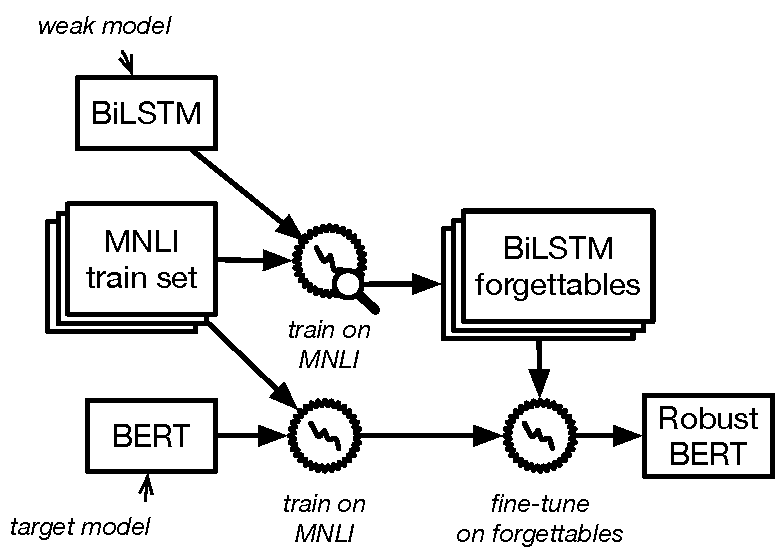
\includegraphics[scale=0.55]{figures/acl.pdf}
\caption{Proposed training for obtaining more robust natural language inference models. We first detect~\emph{forgettable}, or~\emph{hard}, examples from the MNLI training set using a weak model. These are likely to be examples that cannot be solved by simple heuristics. Then, after having fine-tuned a target model on the MNLI training set, we perform an auxiliary round of fine-tuning only on the forgettable subset to obtain a more robust model.}
\label{fig:method}
\end{figure}

\subsection{Our method}
We start from pretrained networks like BERT or XLNet.
In Fig \ref{fig:method}, the basic elements of our method is 
shown. 
We first find a set of forgettable examples using a model, 
then upweight those when training our target model by fine-tuning 
exclusively on them after fine-tuning on all examples first.

The model used for computing forgettables could be any  
simple classifier.
We do not design that model manually and since our targeted heuristics are supposed to be very common, most models' forgettables are violating those heuristics, and when we do the second stage of fine-tuning on forgettables, the target model is adapted to more challenging cases. 
Our method does not introduce a new hyperparameters and it is 
simple compared to other related work. 

To compute forgettables, we follow the original work's algorithm \cite{toneva2018empirical}
 and track the number of times each example is forgotten, following the same procedure described in \citet{toneva2018empirical}. In short, an example is forgotten if it goes from being correctly to incorrectly classified during training (because of gradient updates performed on other examples). 

If an example is forgotten at least once or is never learnt during training, we call it ``forgettable''. 
To remove the effect of shifting label distributions, we randomly sample forgettable examples for each label to keep the label distributions uniform
% of the forgettable sets identical to the ones of MNLI or QQP 
(i.e., 33\% from each of the three labels in MNLI and 50\% for the paraphrase label in QQP). 




\section{Results}
\label{sec:eval}
\subsection{MNLI and HANS}
\begin{table*}[ht]
\footnotesize
\centering
\begin{tabular}{llccc}
\toprule
& \textbf{Train examples} & \textbf{HANS} & \textbf{MNLI} & \textbf{Avg.}  \\
\midrule
\small{1} & All & 58.3 & \textbf{84.5} & 71.4        \\
\midrule
\small{2} & \bertbase forgettables $_{\balancedbert}$   & 48.8                     & 38.9                         & 43.9\\
\small{3} & \hspace{0.1cm} Random $_{\balancedbert}$ & 51.9                   & 75.7                         & 63.8\\
\small{4} & BiLSTM forgettables $_{\balancedlstm}$ & 54.0                     & 66.8                         & 60.4 \\
\small{5} & \hspace{0.1cm} Random $_{\balancedlstm}$ & 51.1                   & 79.0                         & 65.1\\
\small{6} & BoW forgettables $_{\balancedbow}$    & 54.1                     & 68.3                         & 61.2 \\
\small{7} & \hspace{0.1cm} Random $_{\balancedbow}$ & 53.9                   & 79.6                         & 66.8\\
\midrule
&\emph{Additional stage of finetuning} \\
\small{8} & All + \bertbase forgettables   & 70.8                     & 81.8                         & 76.3  \\
\small{9} & All + BiLSTM forgettables &  {73.6}                     & 82.4             & {78.0} \\
\small{10} & \hspace{0.1cm} All + Random $_{\balancedlstm}$       & 60.9                     & 84.4                         & 72.7  \\
\small{11} & All + BoW forgettables    & \textbf{73.7}                     & 82.4             & \textbf{78.1} \\
\midrule
&\emph{Additional stage of finetuning (avg${_{\pm std}}$)} \\
\small{8} & All + \bertbase forgettables   
& $67.4_{\pm 2.47}$                     & $82.0_{\pm 0.25}$                         &   \\
\small{9} & All + BiLSTM forgettables 
&  $69.9_{\pm 2.24}$  & $82.7_{\pm 0.25}$             &  \\
\small{11} & All + BoW forgettables    & $70.4_{\pm 2.10}$                     & $82.5_{\pm 0.25}$             &  \\
\midrule
&\emph{From~\citet{clark2019dont}} & & & \\
\small{12} & All & 62.4 & 84.2 & 73.3 \\
\small{13} & All (reweight) & 69.2 & 83.5 & 76.4 \\
\small{14} & Learned Mixin & 64.0 & 84.3 & 74.2\\
\midrule
&\emph{From~\citet{mahabadi2019simple}} & & &  \\
\small{15} & Product of Experts & 66.5 & 84.0 & 75.3     \\
\midrule
&\emph{From~\citet{he2019unlearn}} & & &  \\
\small{15} & DRiFt-HYPO & 67.1 & 84.3 & 75.7     \\
\midrule
&\emph{From~\citet{linzen2019right} and \citet{Nangia_2019}} & & &  \\
\small{16} & Estimated MTurks & 76.0 & 92.0 & 84.0 \\
\bottomrule
\end{tabular}
\caption{Results of \bertbase model trained on different sources of training examples. For each line, the accuracy of the corresponding model is shown on MNLI dev and HANS and the average of the two.  
Line 1 replicates the original \bertbase result~\citep{devlin2018bert}.
% We denote with $\Delta$ the absolute improvement with respect to the standard setting of fine-tuning on all the MNLI examples (first row). 
Lines from 2 to 7 correspond to finetuning only on subsets of MNLI data. The third block of results (lines from 8 to 11) corresponds to first finetuning \bertbase on the entire MNLI data and then performing an additional finetuning stage on selected examples. We also compare performance to the recent baselines of \newcite{clark2019dont} (lines 12 to 14) and \newcite{mahabadi2019simple} (line 15). They obtain slightly higher results for their base model~\textrm{All} but our best model outperforms theirs.}
\label{tab:twoclass}
\end{table*}

\begin{table*}[]
\small
\centering
\begin{tabular}{lccccccc}
\toprule
\textbf{Model} & \multicolumn{3}{c}{\textbf{Entailment}} & & \multicolumn{3}{c}{\textbf{Contradiction}} \\
& \emph{All}    & \emph{High}  & \emph{Low} & & \emph{All}     & \emph{High}    & \emph{Low} \\
\midrule
All & \textbf{84.1}   & \textbf{90.2}   & \textbf{75.8}  & & 84.7    & 85.4    & \textbf{84.3} \\
All + BiLSTM forgettables & 77.9   & 82.6   & 71.5  & & \textbf{85.0}      & \textbf{87.0} & 84.0  \\   
\bottomrule
\end{tabular}
\caption{Fine-grained accuracy results of \bertbase on MNLI dev set before and after finetuning
on forgettables. 
We split the evaluation set into High ($>$ mean) and Low ($<$ mean) word-overlap examples,
where word-overlap is measures under Jaccard Index between hypothesis and premise. 
Finetuning hurts \ent{} results in both High and Low but improves \nent{} on High.
This is in line with the fine-grained results of HANS depicted in Figure \ref{fig:fine_eval_baselines} where all examples have High word-overlap.}
\label{fine_mnli}   
\end{table*}

\begin{figure}[t]
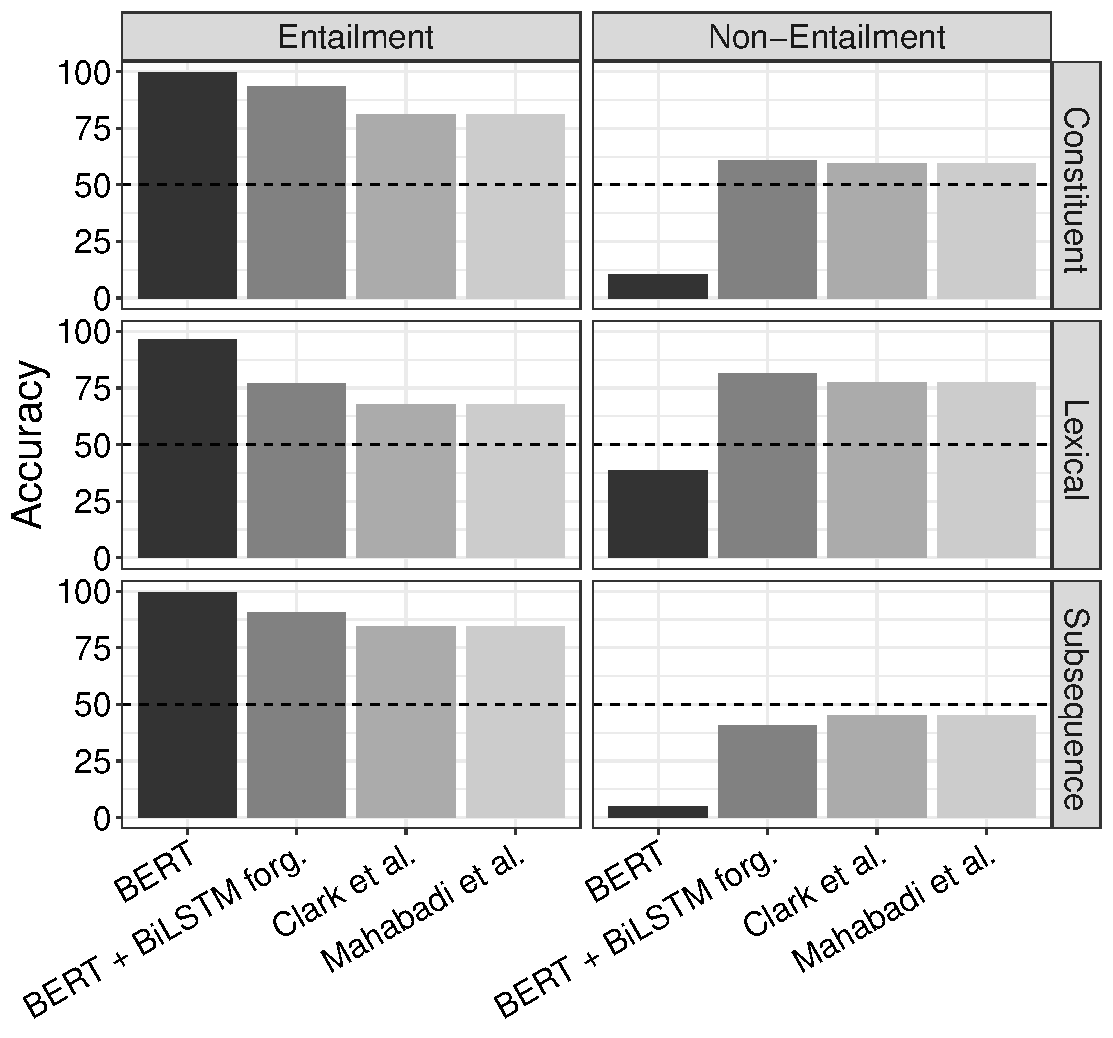
\includegraphics[scale=0.42]{figures/heuristic_plot.pdf}
\caption{Performance of tested models versus the baselines for ``entailment'' and ``non-entailment'' categories and for each heuristic present in the HANS test set. Our approach seems to better retain performance of the entailment category while still increasing accuracy over the baselines of the non-entailment category, albeit to a smaller extent.}
\label{fig:fine_eval_baselines}
\end{figure}


\iffalse
\begin{table}[ht]
\small
\caption{Results of \bertlarge model trained on different sources of training examples.}
\small
\label{tab:bertlarge}
\centering
\begin{tabular}{lccc}
\toprule
\textbf{Train examples} & \textbf{HANS} & \textbf{MNLI} & \textbf{Avg.}  \\
\midrule
All & 72.3 & 86.4 &  79.3 \\
\midrule
\emph{Additional stage of finetuning} & & &\\
All + BoW forgettables & 77.3 & 85.5 & 81.4 \\
All + BiLSTM forgettables & \underline{77.5} & \underline{85.5} & \underline{81.5} \\
\bottomrule
\end{tabular}
\end{table}
\fi

\begin{table*}[ht]
\small
\centering
\begin{tabular}{lcccccc}
\toprule
\textbf{Model} & \multicolumn{2}{c}{\textbf{HANS}} & \multicolumn{2}{c}{\textbf{MNLI}} & \multicolumn{2}{c}{\textbf{Avg.}}  \\
& \emph{base} & \emph{large} & \emph{base} & \emph{large} & \emph{base} & \emph{large} \\
\midrule
BERT & 58.3 & 72.3 & 84.5 & 86.4 & 71.4 & 79.3 \\
BERT + BoW forgettables & 73.7 & 77.3 & 82.4 & 85.5 & 78.1 & 81.4 \\
BERT + BiLSTM forgettables & 73.6 & 77.5 & 82.5 & 85.5 & 78.3 & 81.5 \\
\midrule
XLNET & 63.9$_{\pm 3.0}$ & $76.1_{\pm 2.7}$ & $86.5_{\pm 0.29}$ & 89.7$_{\pm 0.1}$ & & \\
XLNET + BoW forgettables & 73.0 & 85.0 & 84.3 & 88.2 & \\
XLNET + BiLSTM forgettables & 75.1 & 86.8 & 85.5 & 87.8 & &  \\
%\midrule
%Roberta & 46.3 & 50.2 & 87.9 & 89.9 &  & 84.15 \\
%Roberta + BoW forgettables & & & & & \\
%Roberta + BiLSTM forgettables & & & & & & \\
\bottomrule
\end{tabular}
\caption{Results of the \emph{base} and \emph{large} version of various recent NLU models trained on different sources of training examples.}
\label{tab:bertlarge}
\end{table*}



Our main results are presented in Table~\ref{tab:twoclass}.

\paragraph{Forgetting Statistics} Table \ref{tab:forg_stats} shows the number of forgettable examples before and after balancing for BoW, BiLSTM and BERT on MNLI. It is worth noting that the larger the model, the fewer the forgettable examples. The performance of the models on the development set of MNLI is also included, and appears negatively correlated to the number of forgettable examples. Figure~\ref{fig:forgcount-freq} displays the distribution of forgetting events for each model on MNLI, showing in particular the significant number of examples never learnt by our weak baselines.

\paragraph{Training on Forgettables} Lines 2 to 5 report results of fine-tuning BERT on different subsets of the MNLI dataset. This setting aligns with the setting presented in~\citet{toneva2018empirical} where the authors show that, in multiple image classification tasks, the same generalization performance can be obtained by training a model initialized randomly on its own forgettable examples. Our results suggest that this behavior may be task and/or architecture dependent: in our setting, training only forgettable examples particularly affects generalization performance on MNLI. The most extreme drop in performance is observed when BERT is only fine-tuned on its own forgettable examples (line 2) achieving an accuracy of 38.9\%. Training on BiLSTM (line 4) or BoW forgettables (line 6) examples causes a lesser drop in accuracy on MNLI although still noticeable. One of the possible reasons of the dramatic performance loss observed in line 2 is that BERT forgettables are significantly fewer than the counterparts from weaker baselines. 
In order to rule out this hypothesis, we train on a random subset of examples of the same size (\balancedbert, line 3). These results suggest that there is an intrinsic difficulty in BERT forgettables that deserves to be investigated in the future.
To some extent, this is also the case for BiLSTM and BoW forgettables (lines 4 and 6), when comparing to random samples with the same size (lines 5 and 7).

\paragraph{Additional Fine-Tuning} Lines 8-11 report the results obtained by fine-tuning a pretrained model on the set of forgettables, as described in Section \ref{sec:fine_tune}. The results confirm that slightly biasing the model towards hard examples improves robustness at a slight (albeit noticeable) drop in MNLI accuracy. 
Our best model is obtained by using the BiLSTM forgettable examples (line 9) achieving an accuracy of 73.6\% on HANS (max over 3 seeds, mean 73.7\% $\pm$ 0.5\%)
which constitutes a +15.7\% absolute improvement with respect to the base model in line 1 and +4.8\% and +7.5\% with respect to the concurrent models of \newcite{clark2019dont} and \newcite{mahabadi2019simple}. 
Results on line 10 confirm that the forgettables examples identified by BiLSTM are responsible for the improvement: fine-tuning on the same number of randomly chosen examples leads to a much smaller increase. 
Fine-tuning on BoW forgettables (line 11) is also comparable to BiLSTM forgettables (line 9).
% This shows that the choice of the weak model does not seem to matter and therefore prior knowledge about the dataset biases is not required.
An additional observation is that BERT forgettables provide less improvement in robustness than BiLSTM or BoW. 
We hypothesize that this is due to the smaller size of the BERT forgettables compared to BiLSTM or BoW.
% This seems to align with our hypothesis that weaker baselines capture simpler explanations in the dataset.

\textcolor{red}{NEED TO COMMENT ON TABLE 3. We also show the detailed results of HANS based on its three different heuristics for our best performing model (line 9) in Figure \ref{fig:fine_eval_baselines}. 
To give an example of how the various models perform, we retrieved the nearest neighbors of a given HANS example (see Appendix, Table \ref{tab:NNs}).}



\paragraph{Robustness of XLNET and larger models}
\textcolor{red}{\citet{yang2019xlnet} recently introduced XLNET, a transformer-based language model outperforming BERT in standard benchmarks. We applied our evaluation procedure to XLNET and report the results in Table \ref{tab:bertlarge}. \xlnetbase reaches 63.9\% on HANS. After fine-tuning on BiLSTM forgettables, we see an increase of +11.2\%; our method seems to transfer to other architectures.}

\textcolor{red}{Perhaps more interesting, is the effect of using even bigger models. A growing body of literature suggests that increasing the capacity of deep networks results in better generalization \cite{belkin2018reconciling,deepdouble}. These results usually assume no distribution shift between train and test sets. We investigate here whether robustness to the distribution shift studied in this paper may appear ``for free'' in models with a larger number of parameters. To that end, we apply our method to the ``large'' version of BERT and XLNET, \bertlarge and \xlnetlarge, which 
achieve very strong performance on the MNLI dataset~\cite{devlin2018bert,yang2019xlnet}. Results are also shown in Table~\ref{tab:bertlarge}. We see that the large versions generalize on HANS significantly better than their base counterparts (e.g. 76.1\% vs 63.9\% for XLNET), confirming -- in this setting -- that larger models seem more robust. We also observe a significant improvement in performance as a result of finetuning on BiLSTM forgettables, supporting the applicability of the method to larger architectures. In particular, \xlnetlarge fine-tuned on BiLSTM forgettables shows a +10.7\% increase in performance, reaching an impressive 86.8\%!}

\iffalse
\begin{table*}[t]
    \centering
\setlength{\tabcolsep}{4pt}
\begin{tabular}{lcrrrrrrr}
\toprule
\multirow{2}{*}{Training examples} 
&
& \multicolumn{2}{c}{lexical} & \multicolumn{2}{c}{subseq} & \multicolumn{2}{c}{const} \\
     \cmidrule(lr){3-4} \cmidrule(lr){5-6} \cmidrule(lr){7-8}
     & overall 
            & \ent            & \nent           & \ent            & \nent           & \ent             & \nent \\
\midrule
All  & 58.3     
& \bt{0.0}{96.3} & \bt{0.0}{38.4} 
& \bt{0.0}{99.6} & \bt{0.0}{4.7} 
& \bt{0.0}{99.7} & \bt{0.0}{10.6} \\
All + finetuning on BiLSTM forgettables & 73.6   
& \bt{0.0}{76.9} & \bt{0.0}{81.6} 
& \bt{0.0}{90.6} & \bt{0.0}{40.8} 
& \bt{0.0}{93.3} & \bt{0.0}{60.8} \\
\midrule
\newcite{mahabadi2019simple} & 66.5
& \bt{0.0}{93.5} & \bt{0.0}{61.7} 
& \bt{0.0}{96.3} & \bt{0.0}{19.2} 
& \bt{0.0}{98.4} & \bt{0.0}{30.2} \\
\newcite{clark2019dont}  & 69.2
& \bt{0.0}{67.9} & \bt{0.0}{77.4} 
& \bt{0.0}{84.3} & \bt{0.0}{44.9} 
& \bt{0.0}{81.0} & \bt{0.0}{59.6} \\
\bottomrule
\end{tabular}
\caption{Accuracy of the entailment (\ent) and non-entailment (\nent) classes on HANS for three heuristics:
    lexical overlap (lexical), subsequence overlap (subseq), and constituent overlap (const).
}
\label{tab:hans-detailed}
\end{table*}
\fi

\subsection{QQP and PAWS}
\label{sec:paws}
% QQP (Quora question paraphrase) is a paraphrase detection dataset from Quora questions. 
% Each question pair is labeled by either positive or negative. 
% Performance of strong NLP models is very high on the evaluation sets from this data. 
% Recently, PAWS is introduced \cite{zhang-etal-2019-paws} which is made using back translation and applying heuristics for cleanup. The word overlap in PAWS examples is significantly higher than QQP making it a challenging evaluation set for QQP models.
% For example, the accuracy of BERT trained on QQP is drops from around 91\% to 32\%.

In this section, we report the results of our method applied to QPP (see Section \ref{sec:dataset_qqp}).

\paragraph{Forgetting Statistics} Table \ref{tab:forg_stats} contains the number of forgettable examples for our three defaults models. Interestingly, BiLSTM has more forgettables than BoW even though it reaches a better final performance. The distribution of forgetting events for each model can be found in the appendix, Figure \ref{fig:forgcount-freq-qqp}.

\paragraph{Fine-Tuning on Forgettables} We assess the robustness of our fine-tuned models on PAWS. Results can be found in Table \ref{tab:paws}. \textcolor{red}{TO COMPLETE WITH FULL NUMBERS}. 

\begin{table*}[ht]
\small
\centering
\begin{tabular}{lcccccc}
\toprule
\textbf{Model}                           & \multicolumn{2}{c}{\textbf{QQP $\rightarrow$ QQP}} & \multicolumn{2}{c}{\textbf{QQP $\rightarrow$ PAWS}} &           \multicolumn{2}{c}{\textbf{Avg.}}         \\
                                & Acc           & AUC          & Acc           & AUC          & Acc & AUC \\
%\midrule
%Random (p=0.3624)               & 50    & 58.96 & 56.60 & 41.77 & 53.30 & 50.365 \\
%Random (p=0.5)                  & 49.79 & 62.23 & 50.52 & 46.67 & 50.16 & 54.45 \\
%Random (p=0.6376)               & 50    & 66.04 & 43.40 & 50.68 & 46.70 & 58.36 \\
\midrule
% FROM PAWS PAPER, TABLE 7:
\emph{From~\citet{zhang-etal-2019-paws}} \\
BOW                                          & 83.2 & 89.5 & 29.0 & 27.1 & 56.1 & 58.3 \\
BiLSTM                                       & 86.3 & 91.6 & 34.8 & 37.9 & 60.6 & 64.8 \\
ESIM~\citep{chen-etal-2017-enhanced}         & 85.3 & 92.8 & 38.9 & 26.9 & 62.1 & 59.9 \\
DecAtt~\citep{parikh-etal-2016-decomposable} & 87.8 & 93.9 & 33.3 & 26.3 & 60.6 & 60.1 \\
DIIN~\citep{gong2017natural}                 & 89.2 & 95.2 & 32.8 & 32.4 & 61.0 & 63.8 \\
BERT~\citep{devlin2018bert}                  & 90.5 & 96.3 & 33.5 & 35.1 & 62.0 & 65.7 \\
\midrule
\bertbase                       & 90.6 & 96.6 & 32.2 & 33.8 & 61.4 & 65.2 \\
\bertbase + BOW forgettables    & 88.8 & 95.4 & 44.8 & 36.4 & 66.8 & 65.9 \\
\bertbase + BiLSTM forgettables & 88.2 & 95.2 & 41.9 & 37.2 & 65.1 & 66.2 \\
\bertbase + BERT forgettables   & 87.7 & 95.2 & 48.4 & 34.4 & 68.1 & 64.8 \\
\midrule
\bertlarge                       & 91.1 & 96.9 & 34.6 & 35.1 & 62.9 & 66.0 \\
\bertlarge + BiLSTM forgettables & 87.3 & 94.1 & 55.2 & 35.8 & 71.3 & 65.0 \\
\midrule
\xlnetbase                       & 90.9 & 96.6 & 36.6 & 37.5 & 63.8 & 67.1 \\
\xlnetbase + BOW forgettables    & 88.5 & 95.1 & 52.9 & 39.3 & 70.1 & 67.2 \\
\xlnetbase + BiLSTM forgettables & 87.9 & 95.0 & 49.5 & 40.5 & 68.7 & 67.8 \\
\xlnetbase + BERT forgettables   & 88.6 & 95.2 & 60.4 & 38.1 & 74.5 & 66.6 \\
\midrule
\xlnetlarge                       & {91.6} & 97.0   & 49.6 & 43.4 & 70.6 & 70.2 \\
\xlnetlarge + BOW forgettables    & 87.2 & 93 & 68.9 & 50.1 & 78.1 & 71.6\\
\xlnetlarge + BiLSTM forgettables & 85.6 & 92.6 & 64.7 & 52.5 & 75.2 & 72.6\\
\bottomrule
\end{tabular}
\caption{Accuracy (\%) and AUC score (\%) of precision-recall curves are reported for QQP test set and PAWS\textsubscript{QQP} development set. {QQP $\rightarrow$ PAWS} indicates training on QQP and evaluation on PAWS. Results of the \emph{base} and \emph{large} versions of various recent NLU models trained on different sources of training examples. \soroush{I put the 1st seed in this table for base mdoels.} }
\label{tab:paws}
\end{table*}

\begin{table*}[]
\small
\centering
\begin{tabular}{lccc|ccc}
                                & \multicolumn{3}{c|}{\pph} & \multicolumn{3}{c}{\npph} \\

                                & All    & High   & Low   & All     & High    & Low     \\
\toprule

All                       &    &    &   &     &     &     \\
All + BiLSTM forgettables &    &    &   &     &     &     \\   
\bottomrule
\end{tabular}
\caption{Fine-grained accuracy results of \bertbase on QQP dev set before and after finetuning on forgettables. 
We split the evaluation set into High ($>$ mean) and Low ($<$ mean) word-overlap examples,
where word-overlap is measures under Jaccard Index between two sentences. 
%COPIED FROM TABLE 3 fine_mnli: Finetuning hurts \pph{} results in both High and Low but improves \npph{} on High.
%This is in line with the fine-grained results of HANS depicted in Figure \ref{fig:fine_eval_baselines} where all examples have High word-overlap.
}
\label{fine_qqp}   
\end{table*}



\iffalse
\section{Analysis}
\subsection{Final loss as the measure of hardness}
An alternative way of finding hard sets without any prior information is
to simply rank training examples based on their final loss values.
Here, we analyze that and compare with our approach.

One issue with picking examples with loss is that we need to find a threshold value for loss and 
keep only examples with loss value smaller that the threshold.
In this graph we show that the optimum value of this threshold is 
close to the size of forgettables.


\begin{figure}
    \centering
    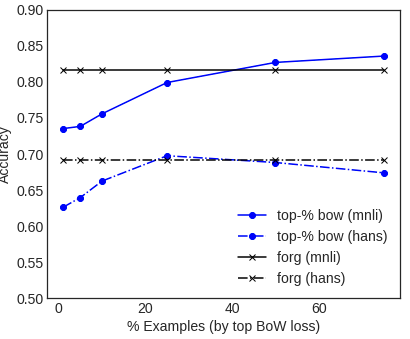
\includegraphics[width=0.5\textwidth]{figures/loss_vs_forg.png}
    \caption{Accuracy on MNLI and HANS when the finetuning set is picked
    from examples in forgettables or in a range of percentages of examples with highest loss.}
    \label{fig:loss_forg}
\end{figure}




\fi

\section{Discussion and Conclusion}
In this paper, we introduce a novel approach based on example forgetting to build more robust models for natural language inference tasks. Via example forgetting, we build a set of hard examples on which a pre-trained MNLI or QQP  model is fine-tuned. When evaluated on the HANS and PAWS out-of-distribution test sets, BERT and XLNET models show a consistent improvement in robustness. We also prove that the larger versions both outperform the base ones and additionally benefit from our method. We discuss next various open questions left for future work.

The abysmal performance of BERT on the MNLI validation set when trained exclusively on its own forgettable examples suggests that \fbert has interesting characteristics. In particular, we highlight the fact that those same examples provide useful learning signal for improving HANS performance when used as an additional fine-tuning stage, but seem to completely lead the model astray when used as the sole training source. This indicates complex interactions between training examples, as well as intricate learning dynamics, which could be better understood using recent advances in deep learning theory, in particular the recent kernel view on deep networks~\citep{jacot2018neural}.

% Fourth, the fact that training on the whole dataset prior to fine-tuning is required (vs simply training on the forgettables) indicates complex interactions between training examples, as well as intricate learning dynamics. Recent advances in deep learning theory, in particular the recent kernel view on deep networks, could help understand our observations better.

% More generally, studying in depth the various forgetting sets might lead to interesting insights.

% Second, while this paper focuses on natural language inference, we conjecture that the method could be applicable to other tasks. A possibility is to test the method on a reading comprehension task such as SQuAD~\cite{rajpurkar2016squad} and tested on adversarial SQuAD~\cite{jia2017adversarial}. 

The experiments showed that our robustness gains are accompanied by a drop in performance on MNLI and QQP.  Although out-of-distribution gains outweigh in-distribution losses (e.g. +12.5\% vs \mbox{-1.9\%} for BERT + \fbow on HANS and MNLI respectively), % but still worth significant attention.
this apparent trade-off seems to be at odds with the goal of simultaneously achieving generalization improvements in- and out-of-distribution. One potential mitigation solution could be to use more sophisticated curriculum learning approaches: smoother ordering of examples, revisiting and/or up-weighting forgettables during training, as is done e.g. in~\citet{clark2019dont,he2019unlearn}. It is however unclear what the limits of this approach are. A future direction would also study the approach more formally in the context of importance weighted empirical risk minimization~\citep{sugiyama2007covariate}.

Finally, we showed that in the considered tasks, larger models are more robust. A related question is to understand why XLNET outperforms BERT on HANS quite significantly. Is it a consequence of the different losses, training data, both?

% current dataset cannot cover well all the modes of the natural lanaguage entailment distribution. under-represented modes, rare events
% fine-tuning on hard BERT and getting better robustness IS a contribution

% Finally, we will study smoother re-weighting of the training examples .

% In this paper, we introduced a novel approach based on example forgetting to build more robust models for a natural language inference task. We  fine-tuned a pre-trained model on a set of ``hard'' examples selected by measuring ``example forgetting''~\citep{toneva2018empirical}. We evaluated the robustness of our approach by training exclusively using the MNLI dataset and the evaluating the model on the out-of-distribution test set of HANS~\citep{linzen2019right}. We improve \bertbase and \bertlarge performance on the challenging HANS test set by more than 15\% and 5\%, respectively. Although this paper focused on natural language inference, the method is widely applicable in other tasks and contexts. This constitutes one possible direction for future work. Moreover, we plan to analyze the forgettable examples more thoroughly to understand their special properties. Finally, we will study smoother re-weighting of the training examples and re-interpret the studied approach more formally in the context of importance weighted empirical risk minimization~\citep{sugiyama2007covariate}.

% \item investigate differences between hard examples and most forgotten examples 
%     \item smoothly integrate the fine-tuning phase by softly reweighting examples
%     \item compute more explicit measures of correlation between forgettables and the biases

%     \item can we even learn to avoid biases if no example contain counter examples of those biases ? put this in discussion

% XLNET vs BERT is it data ? is it the loss ? these questions should be put in discussion
% Drop in MNLI to comment
% understand why BERT forgettables suck.
% what's the tradeoff between MNLI generalization performance and out-of-distribution performance ?
% current dataset cannot cover well all the modes of the natural lanaguage entailment distribution. under-represented modes, rare events
% Just FORG does not work, the combination ALL + FORG does. Interesting in itself, hard to explain, avenue for future research
% fine-tuning on hard BERT and getting better robustness IS a contribution




\section{Related Works}

\paragraph{Curriculum Learning and Sample Weighting}
Curriculum learning is a paradigm that favors learning along a curriculum of examples of increasing difficulty~\citep{bengio2009curriculum}. This general idea has found success in a variety of areas since its introduction~\citep{Kumar10,lee2011learning,schaul2015prioritized}.~\citet{Kumar10} implemented their curriculum by considering easy the examples with a small loss. In our experiments, we empirically validate that unforgettable examples can be safely removed without compromising generalization.~\citet{Zhao2015,conf/icml/KatharopoulosF18} relate sample importance to the norm of its loss gradient with respect to the parameters of the network.~\citet{Fan2017,screenerNet,jiang18mentor} learn a curriculum directly from data in order to minimize the task loss.~\citet{jiang18mentor} also study the robustness of their method in the context of noisy examples. This relates to a rich literature on outlier detection and removal of examples with noisy labels~\citep{john1995robust,brodley1999identifying,sukhbaatar2014training,jiang18mentor}. We will provide evidence that noisy examples rank higher in terms of number of forgetting events. \cite{conf/icml/KohL17} borrow influence functions from robust statistics to evaluate the impact of the training examples on a model's predictions.

\paragraph{Deep Generalization} The study of the generalization properties of deep neural networks when trained by stochastic gradient descent has been the focus of several recent publications~\citep{zhang2016understanding, keskar2016large, Chaudhari2016,Advani2017HighdimensionalDO}. These studies suggest that the generalization error does not depend solely on the complexity of the hypothesis space. For instance, it has been demonstrated that over-parameterized models with many more parameters than training points can still achieve low test error~\citep{huang2017densely,Wang2018} while being complex enough to fit a dataset with completely random labels~\citep{zhang2016understanding}.
A possible explanation for this phenomenon is a form of implicit regularization performed by stochastic gradient descent: deep neural networks trained with SGD have been recently shown to converge to the maximum margin solution in the linearly separable case~\citep{Soudry2017,separable2}. In our work, we provide empirical evidence that generalization can be maintained when removing a substantial portion of the training examples and without restricting the complexity of the hypothesis class. This goes along the support vector interpretation provided by \citet{Soudry2017}.

% \paragraph{Continual Learning} \alex{If Maryia get good results, dump some stuff on continual learning, we'd need also to change the intro to make it a bit more concrete!}.

% \begin{itemize}
%    \item https://arxiv.org/pdf/1801.00904.pdf @\textbf{Remi}, here they apply the stuff they do to reinforcement learning in place of the PER (prioritized experience replay). I think it will be worth thinking about it.
%    \begin{itemize}
%        \item 2016: https://arxiv.org/pdf/1606.04232.pdf hard-removal of examples in the training set in the context of noisy labels. Model obtains low accuracy on MNIST, even lower than removing random subsets of the training set. Their model obtains $~93\%$ test accuracy using $3000$ training samples, whereas we have found that retaining $3000$ random examples for training results in a mean accuracy of $98.02\%$ across $3$ seeds with standard deviation of $0.07$. In comparison, our approach of retaining the most forgotten $3000$ examples results in $98.9\%$ accuracy.
%        \item 1999 https://arxiv.org/pdf/1106.0219.pdf identification of noisy labels , nice discussion about the difference between "noise" (to filter) and "exceptions" (to retain)
% \end{itemize}
% \end{itemize}

\clearpage
\bibliography{bibliography}
\bibliographystyle{acl_natbib}

\appendix
% \section{Detailed results on HANS}
\label{sec:detailedresults}
% \newcommand\ent{$E$}
% \newcommand\neu{$N$}
% \newcommand\con{$C$}
% \newcommand{\nent}{$\neg E$}
% \newcommand{\bt}[2]{#2}

\begin{table*}[t]
\begin{tabular}{p{\textwidth}}
\toprule
\textbf{Source HANS example} \vspace{1mm} \\
\hspace{2mm} \emph{The banker thanked the tourist.} $\longarrownot\longrightarrow$ \emph{The tourist thanked the banker.} \\
\\
\textbf{Nearest neighbors by BERT} \vspace{1mm} \\
\hspace{2mm} \emph{The model simulates the size of the pool of exchangeable base cations in the soil.} \\ \hspace{2mm} $\longrightarrow$ \emph{The model simulates the size of the pool of base cations in the dirt.} \vspace{2mm} \\
\hspace{2mm} \emph{(Or click to read my summary of Wolfe's and Rose's positions.)} \\
\hspace{2mm} $\longrightarrow$ \emph{To read my summary of Wolfe's position, click.} \\
\\
\textbf{Nearest neighbors by our Robust BERT} \vspace{1mm} \\
\hspace{2mm} \emph{He sat patiently as she talked}. $\longarrownot\longrightarrow$
\emph{She sat patiently as he spoke} \vspace{2mm} \\
\hspace{2mm} \emph{And Gates and Appiah would have to be thanked for opening the door.} \\ \hspace{2mm} $\longarrownot\longrightarrow$
\emph{Gates and Appiah were thanked for opening the door.} \\
\bottomrule
\end{tabular}
\caption{Two nearest neighbors for one HANS non-entailment ($\longarrownot\longrightarrow$)  example show-casing how our robust model (line 10 in Table 2) pushes supporting $\longarrownot\longrightarrow$ training data closer compared to standard BERT (MNLI). 
To compute nearest neighbors from the BERT models, the embedding  of the special token (CLS) is assumed as the representation of an example and cosine is used as the similarity metric.}
\label{tab:NNs}
\end{table*}

\iffalse
\begin{table*}[]
\begin{tabular}{p{0.45\textwidth} p{0.45\textwidth} }
\\
\multicolumn{2}{l}{\emph{The HANS example}}
\\
\toprule
\multicolumn{2}{l}{
\begin{tabular}[c]{@{}l@{}}
\emph{The banker thanked the tourist.} $\longarrownot\longrightarrow$ \emph{The tourist thanked the banker.} \\
\end{tabular}
}
\\
\toprule
\multicolumn{1}{c}{\textbf{Nearest neighbors of BERT (MNLI)}}
& \multicolumn{1}{c}{\textbf{Nearest neighbors of our Robust BERT}}     \\
\midrule
\begin{tabular}[t]{@{}p{0.45\textwidth}@{}}
\emph{The model simulates the size of the pool of exchangeable base cations in the soil.} $\longrightarrow$ \emph{The model simulates the size of the pool of base cations in the dirt.} \\
% \\ \emph{Label}: \ent
\end{tabular} & 
\begin{tabular}[t]{@{}p{0.45\textwidth}@{}}
\emph{He sat patiently as she talked}. $\longarrownot\longrightarrow$
\emph{She sat patiently as he spoke}
\end{tabular}
\
\\
% \cmidrule(lr){2-2}
\midrule
\begin{tabular}[c]{@{}p{0.45\textwidth}@{}}
P:	(Or click to read my summary of Wolfe's and Rose's positions.)
H:	To read my summary of Wolfe's position, click.
label: \ent
\end{tabular}
&
\begin{tabular}[c]{@{}p{0.45\textwidth}@{}}
\emph{And Gates and Appiah would have to be thanked for opening the door.} $\longarrownot\longrightarrow$
\emph{Gates and Appiah were thanked for opening the door.} \\
\end{tabular}
\\
\end{tabular}
\caption{Two nearest neighbors for one HANS non-entailment (\nent{})  example show-casing how our robust model (line 10 in Table 2) pushes supporting \nent{} training data closer compared to standard BERT (MNLI). 
To compute nearest neighbors from the BERT models, the embedding 
of the special token (CLS) is assumed as the representation of
an example and cosine is used as the similarity metric.}
\label{tab:NNs}
\end{table*}
\fi


\begin{table*}[]
\small
\centering
\begin{tabular}{lccccccc}
    & \multicolumn{3}{c}{\textbf{Paraphrase}} & & \multicolumn{3}{c}{\textbf{Non-Paraphrase}} \\

                            Model    & \emph{All}    & \emph{High}   & \emph{Low}   & & \emph{All}     & \emph{High}    & \emph{Low}     \\
\toprule

BERT                       & \textbf{90.0} & \textbf{90.8} & \textbf{88.9} &  & 92.2 & 85.6 & 95.0 \\
BERT + \flstm & 85.2 & 84.9 & 85.8 &  & \textbf{93.0} & \textbf{87.3} & \textbf{95.4} \\   
BERT + \fbow    & 87.3 & 87.2 & 87.4 &  & 92.6 & 86.4 & 95.2 \\   
\bottomrule
\end{tabular}
\caption{Fine-grained accuracy results of BERT on QQP development set before and after finetuning on forgettables. 
We split the evaluation set into High ($>$ mean) and Low ($<$ mean) word-overlap examples,
where word-overlap is measures under Jaccard Index between two sentences. Similar observations than in the case of MNLI hold.
%COPIED FROM TABLE 3 fine_mnli: Finetuning hurts \pph{} results in both High and Low but improves \npph{} on High.
%This is in line with the fine-grained results of HANS depicted in Figure \ref{fig:fine_eval_baselines} where all examples have High word-overlap.
}
\label{fine_qqp}   
\end{table*}

%\begin{figure}[t]
%\centering
%  \includegraphics[width=0.45\textwidth]{figures/ex_by_forg_qqp.png}
%  \caption{Distribution of forgetting events for the three models after five training epochs on QQP. }
%\label{fig:forgcount-freq-qqp}
%\end{figure}

\end{document}

%TODO:
%- https://dawn.cs.stanford.edu/2019/03/22/glue/ (Signal 4: Dataset Slicing) 

% https://microsoft-my.sharepoint.com/:x:/r/personal/yayaghoo_microsoft_com/_layouts/15/Doc.aspx?sourcedoc=%7B41975454-abff-488b-8f55-c550ad840d9f%7D&action=edit&activeCell=%27compare_baseModels%27!D9&wdInitialSession=c219a303-a524-465a-bdd6-28ac21d1312c&wdRldC=1

% \begin{table}[h]
%     \centering
%     \begin{tabular}{l | l l}
%         Train source & HANS & MNLI \\
%         \hline
%         All & 60.0 & \\
%         BERT forgettables & & \\
%         BiLSTM forgettables                       & 54.0 & \\
%         BiLSTM forgettables + 20\% unforgettables & 57.5 & \\
%         BiLSTM forgettables + 30\% unforgettables & 57.5 & \\
%         BiLSTM forgettables + 50\% unforgettables & 57.5 & \\
%         BiLSTM forgettables + 80\% unforgettables & 57.5 & \\
%         \hline 
%         pretrian all, fine-tune on BERT forgettables & 67.8 & \\
%         pretrian all, fine-tune on BiLSTM forgettables & 69.2 & \\
%         pretrian all, fine-tune on BiLSTM 20\% unforgettables & 61.7 & \\
        
%     \end{tabular}
%     \caption{Caption}
%     \label{tab:my_label}
% \end{table}

